%! Author = kucera-lukas
%! Date = 4/13/22

\section{Ostatní}\label{sec:ostatni}

\subsection{Barevný motiv}\label{subsec:barevny-motiv}
Aplikace umožňuje změnu barevného motivu.
Stačí kliknout na ikonku v pravém horním rohu.

\begin{figure}
    \centering
    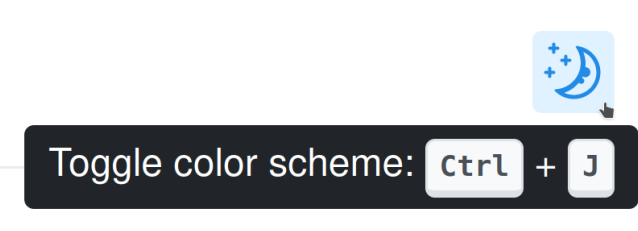
\includegraphics[scale=0.4]{assets/images/color-scheme}
    \caption{Barevný motiv}\label{fig:barevny-motiv}
\end{figure}

\subsubsection{Klávesová zkratka}
Barevný motiv lze také přepnout klávesovou zkratkou \texttt{ctrl + k}.

\subsubsection{Lokální úložistě}
Vybraný motiv se uloží do \texttt{Window.localStorage}
\url{https://developer.mozilla.org/en-US/docs/Web/API/Window/localStorage}
a tak není potřeba motiv upravovat při každém vstupu na webovou stránku.
